\include{preambule}

\begin{document}
\begin{titlepage}
	\noindent\begin{minipage}{0.05\textwidth}
		\includegraphics[scale=0.3]{img/bmstu.png}
	\end{minipage}
	\hfill
	\begin{minipage}{0.85\textwidth}\raggedleft
		\begin{center}
			\fontsize{12pt}{0.3\baselineskip}\selectfont \textbf{Министерство науки и высшего образования Российской Федерации \\ Федеральное государственное бюджетное образовательное учреждение \\ высшего образования \\ <<Московский государственный технический университет \\ имени Н.Э. Баумана \\ (национальный исследовательский университет)>> \\ (МГТУ им. Н.Э. Баумана)}
		\end{center}
	\end{minipage}
	
	\begin{center}
		\fontsize{12pt}{0.1\baselineskip}\selectfont
		\noindent\makebox[\linewidth]{\rule{\textwidth}{4pt}} \makebox[\linewidth]{\rule{\textwidth}{1pt}}
	\end{center}
	
	\begin{flushleft}
		\fontsize{12pt}{0.8\baselineskip}\selectfont 
		
		ФАКУЛЬТЕТ \uline{<<\textbf{Информатика и системы управления}>> \hfill}
		
		КАФЕДРА \uline{<<\textbf{Программное обеспечение ЭВМ и информационные технологии}>> \hfill}
	\end{flushleft}
	
	\vfill
	
	\begin{center}
		\fontsize{20pt}{\baselineskip}\selectfont
		
		\textbf{РАСЧЕТНО-ПОЯСНИТЕЛЬНАЯ ЗАПИСКА}
		
		\textbf{\textit{К КУРСОВОМУ ПРОЕКТУ}}
		
		\textbf{\textit{НА ТЕМУ:}}
	\end{center}
	
	\begin{center}
		\fontsize{18pt}{0.6cm}\selectfont 
		
		<<Моделирование зеркального кубика Рубика>>
		
	\end{center}
	
	\vfill
	
	\begin{table}[h!]
		\fontsize{12pt}{0.7\baselineskip}\selectfont
		\centering
		\begin{signstabular}[0.7]{p{7.25cm} >{\centering\arraybackslash}p{4cm} >{\centering\arraybackslash}p{4cm}}
			Студент группы \textbf{ИУ7-56Б} & \uline{\mbox{\hspace*{4cm}}} & \uline{\hfill \textbf{Чепрасов К.М.} \hfill} \\
			& \scriptsize (Подпись, дата) & \scriptsize (И.О. Фамилия)
		\end{signstabular}
		
		\vspace{\baselineskip}
		
		\begin{signstabular}[0.7]{p{7.25cm} >{\centering\arraybackslash}p{4cm} >{\centering\arraybackslash}p{4cm}}
			Научный руководитель & \uline{\mbox{\hspace*{4cm}}} & \uline{\hfill \textbf{Мальцева Д.Ю.} \hfill} \\
			& \scriptsize (Подпись, дата) & \scriptsize (И.О. Фамилия)
		\end{signstabular}
	\end{table}
	
	\vfill
	
	\begin{center}
		\normalsize \textbf{2022} г.
	\end{center}
\end{titlepage}
\setcounter{page}{3}
\tableofcontents
\section*{Введение}
\addcontentsline{toc}{section}{Введение}
Кубик Рубика является очень простой головоломкой с точки зрения своего устройства. Но стоящая за ней математика проделала довольно долгий путь. Существуют нерешённые задачи, связанные с этой головоломкой.

Сам по себе кубик Рубика, может выглядеть очень по-разному. В рамках данного курсового проекта будет рассмотрена одна из вариаций данной головоломки, а именно --- зеркальный кубик Рубика.

Целью курсового проекта является разработка программы построения и визуализации трёхмерной модели зеркального кубика Рубика на основе данных о вращении его граней. Для достижения поставленной цели необходимо решить следующие задачи:
\begin{itemize}
	\item разработка способа формального представления кубика Рубика;
	\item анализ существующих алгоритмов удаления невидимых граней;
	\item реализация описанного алгоритма;
	\item проектирование архитектуры программы;
	\item разработка интерфейса программы;
	\item разработка спроектированного ПО.
\end{itemize}

\section{Аналитический раздел}
\subsection{Кубик Рубика}
Кубик Рубика (в честь Эрнё Рубика) --- механическая головоломка, представляющая из себя куб,
каждая грань которого имеет уникальный цвет и делится малыми кубами на 9 частей (26 в сумме со всех сторон) \cite{bib:how_to_assemble}.
Механизм, располагающийся в центре кубика, позволяет вращать каждую грань относительно кубика Рубика.
Таким образом, набор случайных поворотов граней приводит к «разборке» кубика рубика.
Обратная «сборка» заключается в последовательности поворотов грани так,
чтобы каждая грань кубика рубика снова стала одноцветной.

\begin{figure}[ht]
	\centering
	\includegraphics[width=1\linewidth]{rubicks_cube}
	\caption{Кубик Рубика}
	\label{fig:rubicks_cube}
\end{figure}

\subsubsection{Формализация действий над кубиком Рубика}
В дальнейшем, будем использовать обозначения поворотов граней кубика Рубика, введённые <<World Cube Association>> \cite{bib:cube_notation}. Пусть куб находится напротив наблюдателя. Тогда:

\begin{itemize}
	\item F (front) --- фронтальная грань. Находится непосредственно напротив наблюдателя.
	\item B (back) --- задняя грань. Противоположная фронтальной.
	\item L (left) --- левая грань. Находится по левую руку от наблюдателя.
	\item R (right) --- правая грань. Находится по правую руку от наблюдателя.
	\item U (up) --- верхняя грань.
	\item D (down) --- нижняя грань.
\end{itemize}

Операции поворота грани по часовой стрелке обозначаются именем грани. Так, например, повернуть дважды фронтальную грань, затем повернуть по часовой стрелке верхнюю грань будет обозначаться так: FFU.

Предусмотрено обозначение для поворота грани против часовой стрелки, для этого после символа обозначения грани добавляется апостроф. Так, например, поворот правой грани по часовой стрелке, затем поворот нижней грани против часовой стрелки, затем поворот правой грани по часовой стрелке обозначается так: RD’R.

\begin{figure}[ht]
	\centering
	\includegraphics[width=1\linewidth]{cube_rotations}
	\caption{Способы поворота граней кубика Рубика}
	\label{fig:cube_rotations}
\end{figure}

\subsubsection{Сборка кубика Рубика}
Для сборки кубика Рубика не обязательно знать всю последовательность действий, применённую к нему, достаточно информации о цветах граней. Для сборки кубика Рубика можно применить алгоритм Джессики Фридрих \cite{bib:fridrich}.

Сборка кубика Рубика по методу Джессики Фридрих, делится на четыре этапа:
\begin{enumerate}
	\item Сборка «креста»
	\item Сборка первых двух слоёв (F2L)
	\item Ориентация кубиков верхнего слоя (OLL)
	\item Расстановка кубиков верхнего слоя (PLL)
\end{enumerate}

Каждый из этих этапов имеет конечное, относительно малое количество вариантов расположения цветов граней. Решение очередного этапа кубика Рубика состоит в определении конкретной ситуации (цветов граней), и применение соответствующей последовательности действий. Например, во время сборки OLL может возникнуть ситуация, проиллюстрированная на рис. \ref{fig:c_shape}. Её решением является следующая последовательность действий: R'U'R'FRF'UR

\begin{figure}[ht]
	\centering
	\includegraphics[width=0.25\linewidth]{c_shape}
	\caption{Ситуация, которая может возникнуть во время сборки OLL}
	\label{fig:c_shape}
\end{figure}

\subsubsection{Зеркальный кубик Рубика}
\begin{figure}[ht]
	\centering
	\includegraphics[width=1\linewidth]{mirrored_rubics_cube}
	\caption{Внешний вид зеркального кубика Рубика в собранном (слева) и в разрбранном (справа) состояниях}
	\label{fig:mirrored_cube}
\end{figure}

Цвет --- не единственный способ обозначать правильно собранные грани. Одной из модификаций классического кубика Рубика является зеркальный кубик Рубика. Он отличается от классической версии тем, что грани отличаются не по цвету, а по высоте каждого параллелограмма относительно центра кубика. Грань собранного кубика Рубика состоит из граней параллелограммов разного размера, но остаётся в форме квадрата; при разборке --- форма меняется. Несмотря на эти различия, зеркальная и классическая версии кубика Рубика имеют общие принципы сборки.

\subsubsection{Пропорции зеркального кубика Рубика}
Введём пропорции зеркального кубика Рубика (рисунок \ref{fig:mirrored_cube_proportions}). Пусть:
\begin{itemize}
	\item наблюдатель смотрит по направлению оси X (нормаль к грани B),
	\item строго налево от наблюдателя направлена ось Y (нормаль к грани L),
	\item сторо наверх от наблюдателя направлена ось Z (нормаль к грани U)
\end{itemize}

Тогда вдоль каждой оси последовательно отложим отрезки трёх длин:
\begin{itemize}
	\item для оси X: 17, 19, 21
	\item для оси Y: 13, 19, 25
	\item для оси Z: 9, 19, 29
\end{itemize}

Плоскости, проведённые перпендикулярно соответствующей оси на границе отрезка, отрезают трёхмерный куб размером 57x57x57, разделённый на 27 параллелограммов. 

\begin{figure}[ht]
	\centering
	\includegraphics[width=1\linewidth]{mirrored_cube_propotions}
	\caption{Пропорции зеркального кубика Рубика}
	\label{fig:mirrored_cube_proportions}
\end{figure}

\subsection{Отрисовка сцены}
Одной из основных задач разрабатываемого програмного продукта является отрисовка зеркального кубика Рубика. Рассмотрим существующие алгоритмы удаления невидимых граней:
\begin{itemize}
	\item Алгоритм плавающего горизонта
	\item Алгоритм Варнока
	\item Алгоритм Робертса
	\item Алгоритм Вейлера-Азертона
	\item Алгоритм, Z-буфера
	\item Алгоритм, использующий список приоритетов
	\item Алгоритмы построчного сканирования
\end{itemize}

Все вышеперечисленные алгоритмы не могут привести к корректному результату, если среди объектов сцены присутствует зеркальные поверхности. Таким образом, для отрисовки зеркальных поверхностей необходимо использовать алгоритм трассировки лучей \cite{bib:computergraphics}.

\subsubsection{Алгоритм прямой трассировки лучей}
Основная идея алгоритма --- промоделировать поведение света для получения реалистичного изображения. В реальном мире, свет исходит от источника света, отражается от отражающих поверхностей и рассеивается рассеивающими поверхностями. Некоторые лучи света попадают на сетчатку глаза, которая посылает сигнал об интенсивности и цвете пришедшего луча. Алгоритм, реализующий такую модель, называется алгоритмом прямой трассировки лучей.

\subsubsection{Алгоритм обратной трассировки лучей}
\begin{figure}[ht]
	\centering
	\includegraphics[width=1\linewidth]{backward_ray_trace}
	\caption{Обратная трассировка лучей}
	\label{fig:backward_ray_trace}
\end{figure}

Заметим, что нас интересуют лишь те лучи света, которые попали на сетчатку глаза. На основе этого, при моделировании подобной системы, лучи можно пускать в обратную сторону, то есть начиная от сетчатки. Теперь цвет луча при столкновении будет рассчитываться в зависимости от освещённости очередной точки попадания луча и цвета поверхности, на которую попал луч.

В качестве допущения, будем считать, что все поверхности на сцене являются непрозрачными.

\subsubsection{Описание алгоритма обратной трассировки лучей}
Алгоритму поступает следующие данные:
\begin{itemize}
	\item местополжение наблюдателя;
	\item расстояние до проецирующей плоскости;
	\item местоположение и геометрия всех объектов на сцене.
\end{itemize}

На основе этих данных, алгоритм должен окрасить сетку пикселей $n\times m$ так, чтобы при отображении её на экране, можно было распознать реалистичное изображение.

Для каждого пикселя, из камеры пускается луч в соответствующем направлении. При попадании луча в плоскость, порождается дополнительный луч, отражённый. Вектор отражения $\bar V_M$, при исходном луче $\bar V$, относительно нормали $\bar n$, при $|\bar n| = 1$ считается по следующей формуле:

\begin{equation}
	\bar V_M = \bar V - 2\cdot\bar V \cdot\bar n\cdot\bar n
	\label{eq:bounce}
\end{equation}

Цвет данной точки рассчитывается как смешение цвета поверхности и цвета, рассчитаного при попадании луча $\bar V_M$ на поверхность.

С целью упростить задачу поиска пересечения луча и поверхности, будем считать, что каждый объект сцены можно представить в виде набора из конечного числа треугольников.

\subsection{Вывод по разделу}
В аналитическом разделе был описан кубик Рубика, обозначения граней и их поворотов. Была объяснена разница между классическим кубиком Рубика и его вариацией --- зеркальным кубиком Рубика.

Так же, описана задача отрисовки трёхмерной сцены. Обозначена причина, по которой был выбран алгоритм обратной трассировки лучей в качестве способа отрисовки трёхмерной сцены.

Были установлены ограничения по содержанию сцены, а именно:
\begin{itemize}
	\item Все объекты на сцене являются непрозрачными
	\item Каждый объект сцены можно представить в виде конечного набора треугольников
\end{itemize}


\section{Конструкторский раздел}
Во время разработки программы, должна быть учтена возможность её модификации. Объектно-ориентированный подход обеспечивает гибкость в вопросе изменения уже существующего кода \cite{bib:oop_mod}.

В программы будет высоконагруженная секция --- алгоритм отрисовки сцены. При разработке алгоритма, необходимо как можно больше операций перенести на другие части программы, с целью получения максимального выигрыша в производительности.

\subsection{Сцена, объекты сцены}
Определим ключевые сущности, тем или иным образом связанные с понятием сцены:
\begin{itemize}
	\item Сцена. Должна агрегировать все объекты, которые могут быть включены в неё.
	\item Полигональная модель. Будет содержать множество точек в пространстве и ими задаваемые треугольники.
	\item Камера. Представляет собой точку в пространстве, имеющую направление и область обзора.
	\item Кубик Рубика. Агрегирует 27 моделей малых параллелограммов, формирующих зеркальный кубик Рубика.
\end{itemize}

Добавив несколько вспомогательных классов, получим UML-диаграмму (см. рис. \ref{fig:uml_scene}). Полученая диаграмма описывает некий домен сцены. Рассмотрим основные математические структуры:
\begin{figure}[ht]
	\centering
	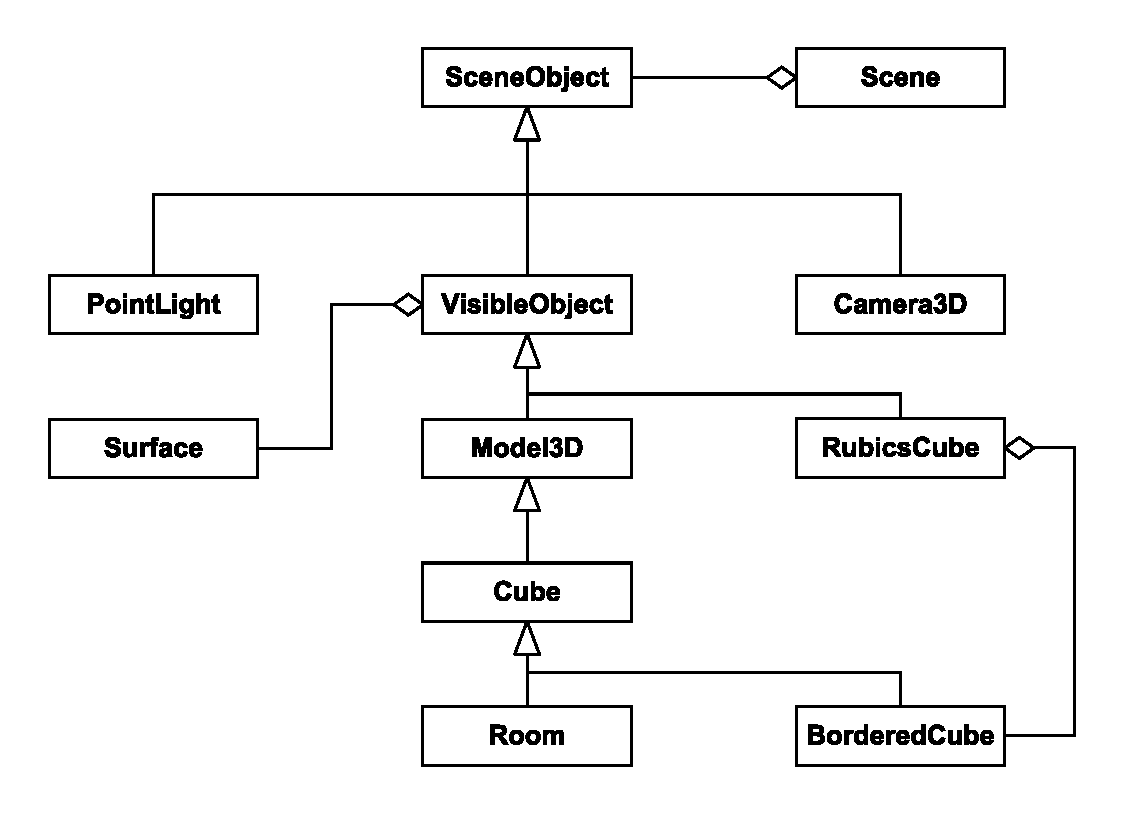
\includegraphics[width=1\linewidth]{uml_scene}
	\caption{UML диаграмма классов сцены, без описания полей и методов}
	\label{fig:uml_scene}
\end{figure}

\subsection{Математические структуры}
Для описания положения объекта в пространстве, необходима следующая информация:
\begin{itemize}
	\item позиция объекта,
	\item поворот объекта,
	\item размер объекта.
\end{itemize}

\subsubsection{Трёхмерный вектор}
Трёхмерный вектор является тройкой действительных чисел $(x, y, z)$, каждая компонента которого является величиной проекции на соответствующую ось \cite{bib:vector}.

Позиция объекта может быть описана радиус-вектором, описывающим смещение всех точек объекта относительно начала координат. Таким образом, достаточно прибавить данный радиус-вектор к каждой точке трёхмерной модели, чтобы получить её истинное положение.

Используя точно такую же структуру, будем обозначить размер объекта. Каждый компонент вектора является коэффициентом масштабирования для каждой оси.

\subsubsection{Кватернион}
Использование тройки углов, описывающих последовательный поворот объекта вдоль всех осей, имеет свои недостатки \cite{bib:euler_problems}:
\begin{itemize}
	\item неоднозначность. Для любой последовательности вращений $A$, существует как минимум одна другая последовательность, приводящая объект к тому-же положению, что $A$;
	\item некорректный результат при последовательном применении двух и более троек углов поворота.
\end{itemize}

Вместо так называемых Эйлеровых углов, предпочтительнее использовать кватернионы \cite{bib:quaternions}.

Кватернион представляет собой кортеж из четырёх чисел $(q_0, q_1, q_2, q_3)$. Для каждого кватерниона $q$, существует обратный ему $q^{-1}\ne q$:
\begin{equation}
	q^{-1}=(q_0, -q_1, -q_2, -q_3),
\end{equation}

исключением является единичный кватернион $(1, 0, 0, 0)$, так как он обратен самому себе.

Для кватернионов определена операция умножения. Пусть:
\begin{equation}
	(t_0, t_1, t_2, t_3) = (r_0, r_1, r_2, r_3)\times(s_0, s_1, s_2, s_3).
\end{equation}

Тогда:
\begin{subequations}
	\begin{align}
		t_0=(r_0\cdot s_0-r_1\cdot s_1-r_2\cdot s_2-r_3\cdot s_3) \\
		t_1=(r_0\cdot s_1+r_1\cdot s_0-r_2\cdot s_3+r_3\cdot s_2) \\
		t_2=(r_0\cdot s_2+r_1\cdot s_3+r_2\cdot s_0-r_3\cdot s_1) \\
		t_3=(r_0\cdot s_3-r_1\cdot s_2+r_2\cdot s_1+r_3\cdot s_0)
	\end{align}
\end{subequations}

С помощью кватерниона, можно повернуть точку в пространстве, заданную тремя координатами. Для этого нужно задать кватернион $p$, как:
\begin{equation}
	p=(p_0,p_1,p_2,p_3)=(0, x, y, z),
\end{equation}
где $(x, y, z)$ - точка в пространстве. Получим $p'$ следующим образом:
\begin{equation}
	p'=q^{-1}\cdot p\cdot q,
\end{equation}
где $q$ --- кватернион, описывающий вращение. Искомая точка является тройкой $(p'_1, p'_2, p'_3)$.

\subsubsection{Цвет}
Структура цвета необходима для описания поверхностей объектов. Представляет собой тройку чисел $(r, g, b)$. Значение компонент определяет интенсивность цветов: красного, зелёного и синего соответственно. Сочетания этих трёх цветов разной интенсивности позволяют получить любой другой цвет.

Определим операцию умножения цвета на скаляр:
\begin{equation}
	C\cdot k=(r, g, b)\cdot k=(r\cdot k, g\cdot k, b\cdot k),
\end{equation}
где $C$ --- исходный цвет, $k$ --- скаляр.

Определим операцию сложения цветов:
\begin{equation}
	C_1+C_2=(r_1, g_1, b_1)+(r_2, g_2, b_2)=(r_1+r_2,g_1+g_2,b_1+b_2),
\end{equation}
где $C_1$ и $C_1$ --- исходные цвета

\subsubsection{Список математических структур}
В конечном итоге, выделяем следующие структуры:
\begin{itemize}
	\item Vector3D --- трёхмерный вектор
	\item Quaternion --- кватернион
	\item Transform --- положение объекта в пространстве
	\item Color --- цвет
\end{itemize}

\subsection{Алгоритм обратной трассировки лучей}
Основная идея алгоритма трассировки лучей заключается в том, чтобы проследить путь, который проходит свет от источника до наблюдателя. Делается этот процесс в обратном направлении, то есть из точки наблюдателя выпускаются лучи, которые, несколько раз отражаются от встреченных поверхностей. Данный процесс продолжается до тех пор, пока либо количество дополнительно выпущеных лучей не превысит определённое значение, либо очередная поверхность не окажется неотражающей.

\subsubsection{Алгоритм определения цвета пикселя}
Алгоритм, определяющий цвет пикселя, принимает на вход два трёхмерных вектора: местонахождение наблюдателя (rs) и направление бросания луча (rd). Схема алгоритма представлена на рис. \ref{fig:calculate_pixel_color}

\begin{figure}[!ht]
	\centering
	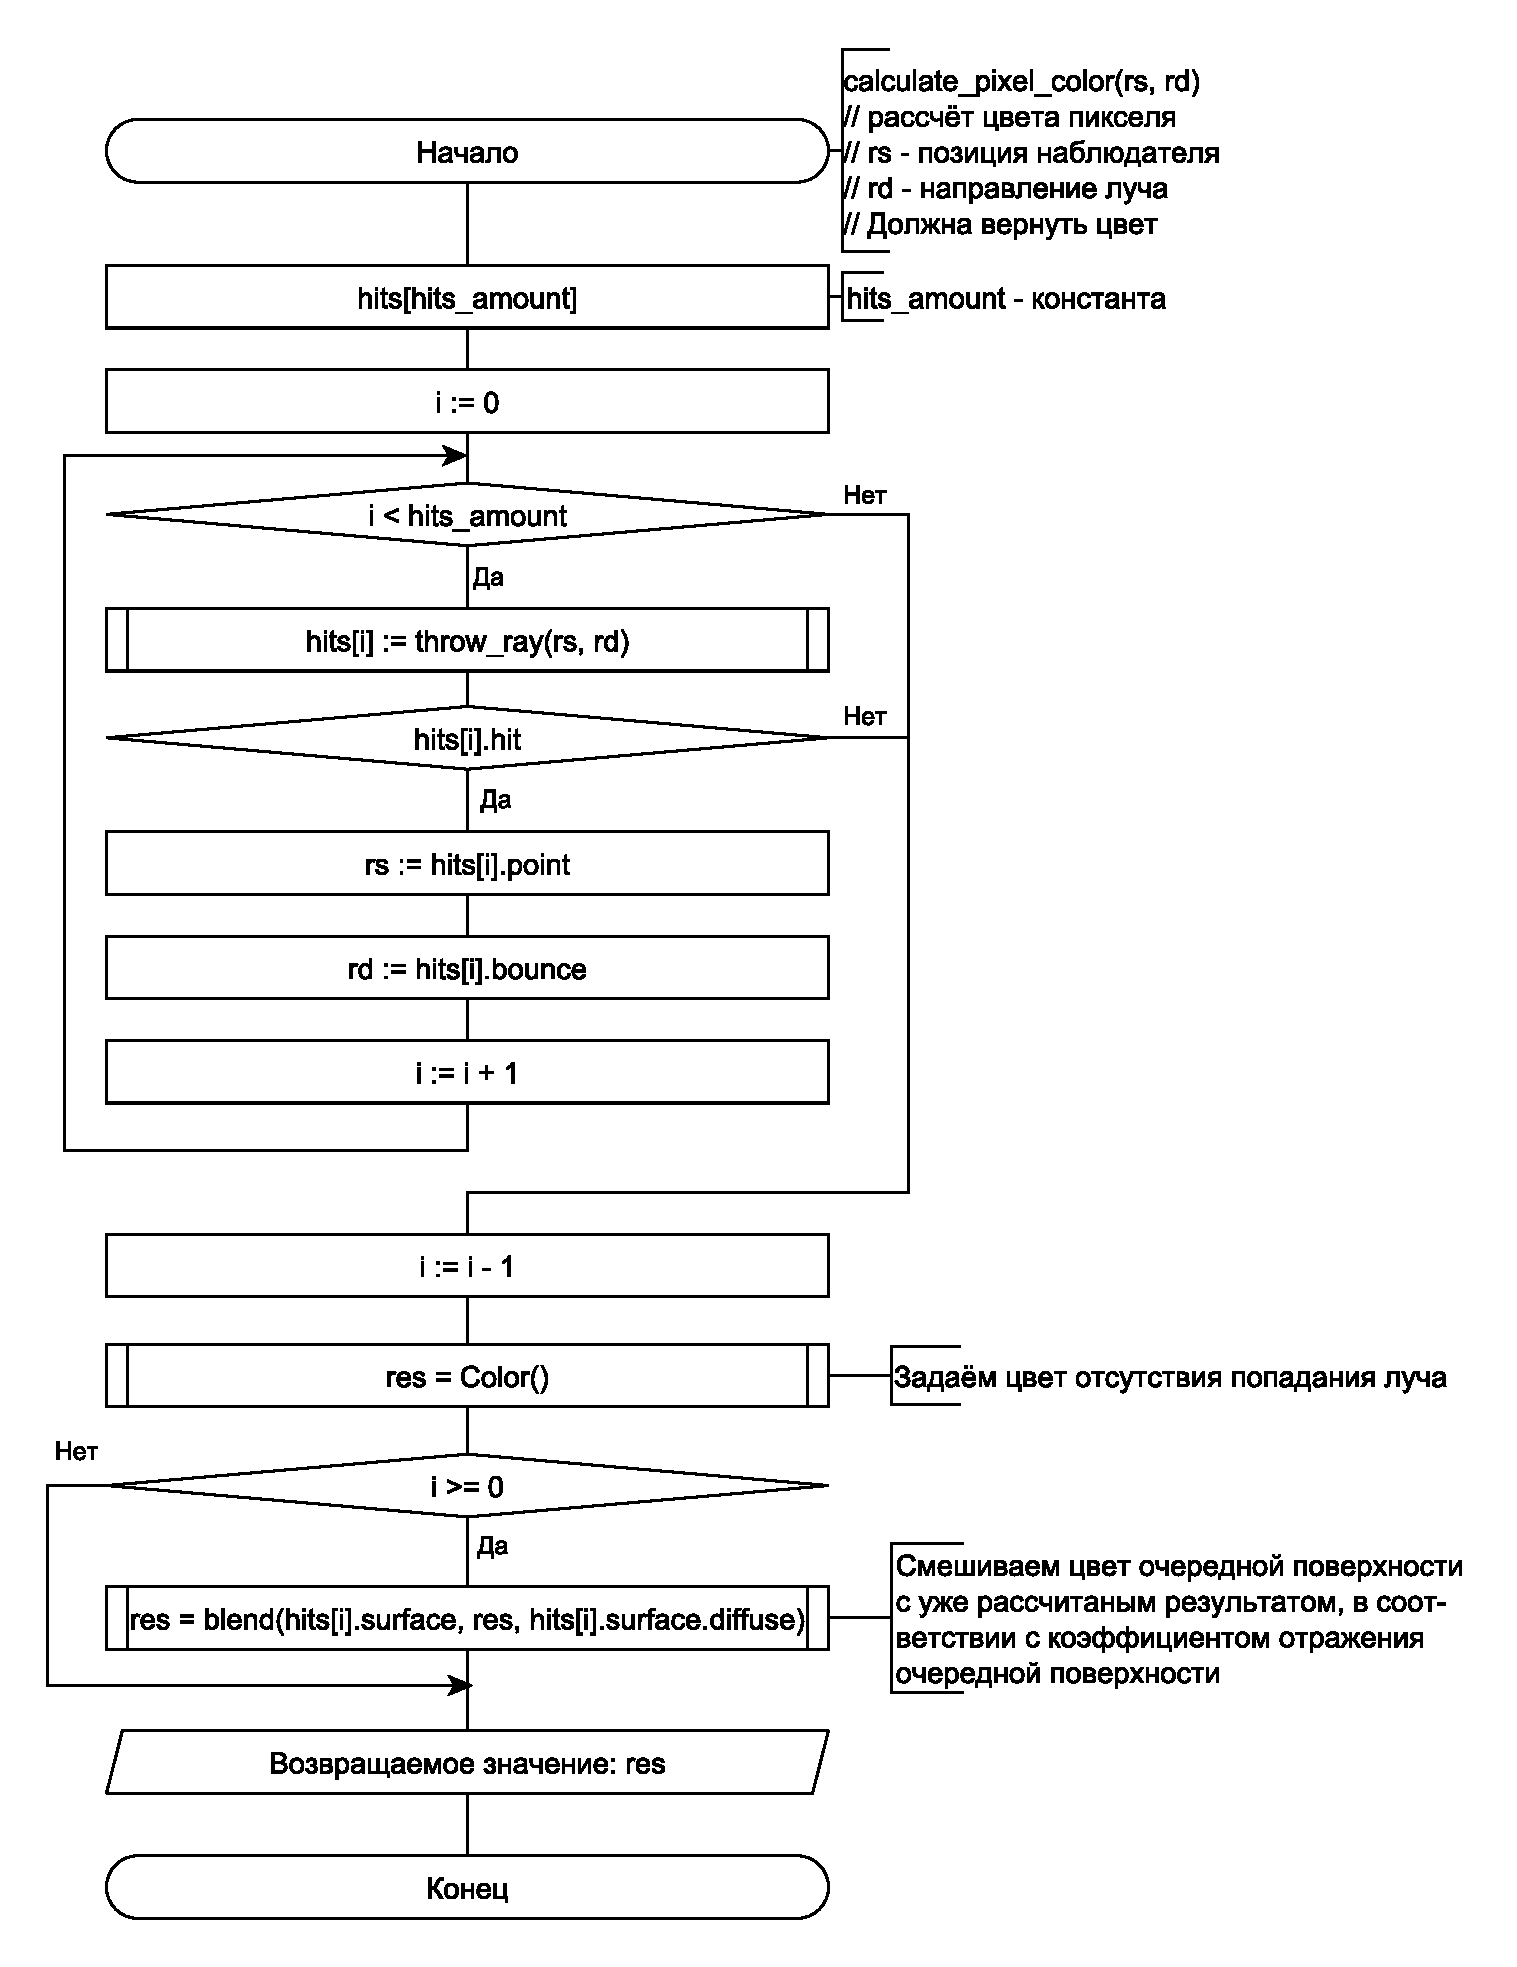
\includegraphics[width=1\linewidth]{calculate_pixel_color}
	\caption{Схема алгоритма определения цвета пикселя}
	\label{fig:calculate_pixel_color}
\end{figure}

Переменная hits[] является массивом из структур, содержащих информацию о попадании. Они должны хранить следующие данные:
\begin{itemize}
	\item было ли попадание (hit) --- логическое;
	\item точке попадания луча (point) --- трёхмерный вектор;
	\item направление отскока (bounce) --- трёхмерный вектор;
	\item поверхность, с которой произошло пересечение (surface) --- поверхность;
\end{itemize}

Структура поверхности содержит в себе информацию о треугольнике в пространстве и его свойствах, а именно:
\begin{itemize}
	\item три точки, задающие треугольник (points) --- тройка трёхмерных векторов;
	\item коэффициент рассеивания (diffuse) --- вещественное. Является обратным к коэффициенту отражения;
	\item цвет поверхности (color) – цвет;
	\item нормаль к поверхности (normal) --- трёхмерный вектор;
	\item объект, частью которого является поверхность (owner) --- объект сцены;
\end{itemize}

Функция Blend реализует смешение двух цветов по формуле:
\begin{equation}
	C = C_1\cdot k+C_2\cdot(1-k),
\end{equation}
где $C$, $C_1$, $C_2$ --- цвета, $k\in[0, 1]$ --- скаляр.

\subsubsection{Алгоритм бросания луча}
Алгоритм бросания луча принимает на вход два трёхмерных вектора: местонахождение наблюдателя (rs) и направление бросания луча (rd). Схема алгоритма представлена на рис. \ref{fig:throw_ray}.

\begin{figure}[!ht]
	\center{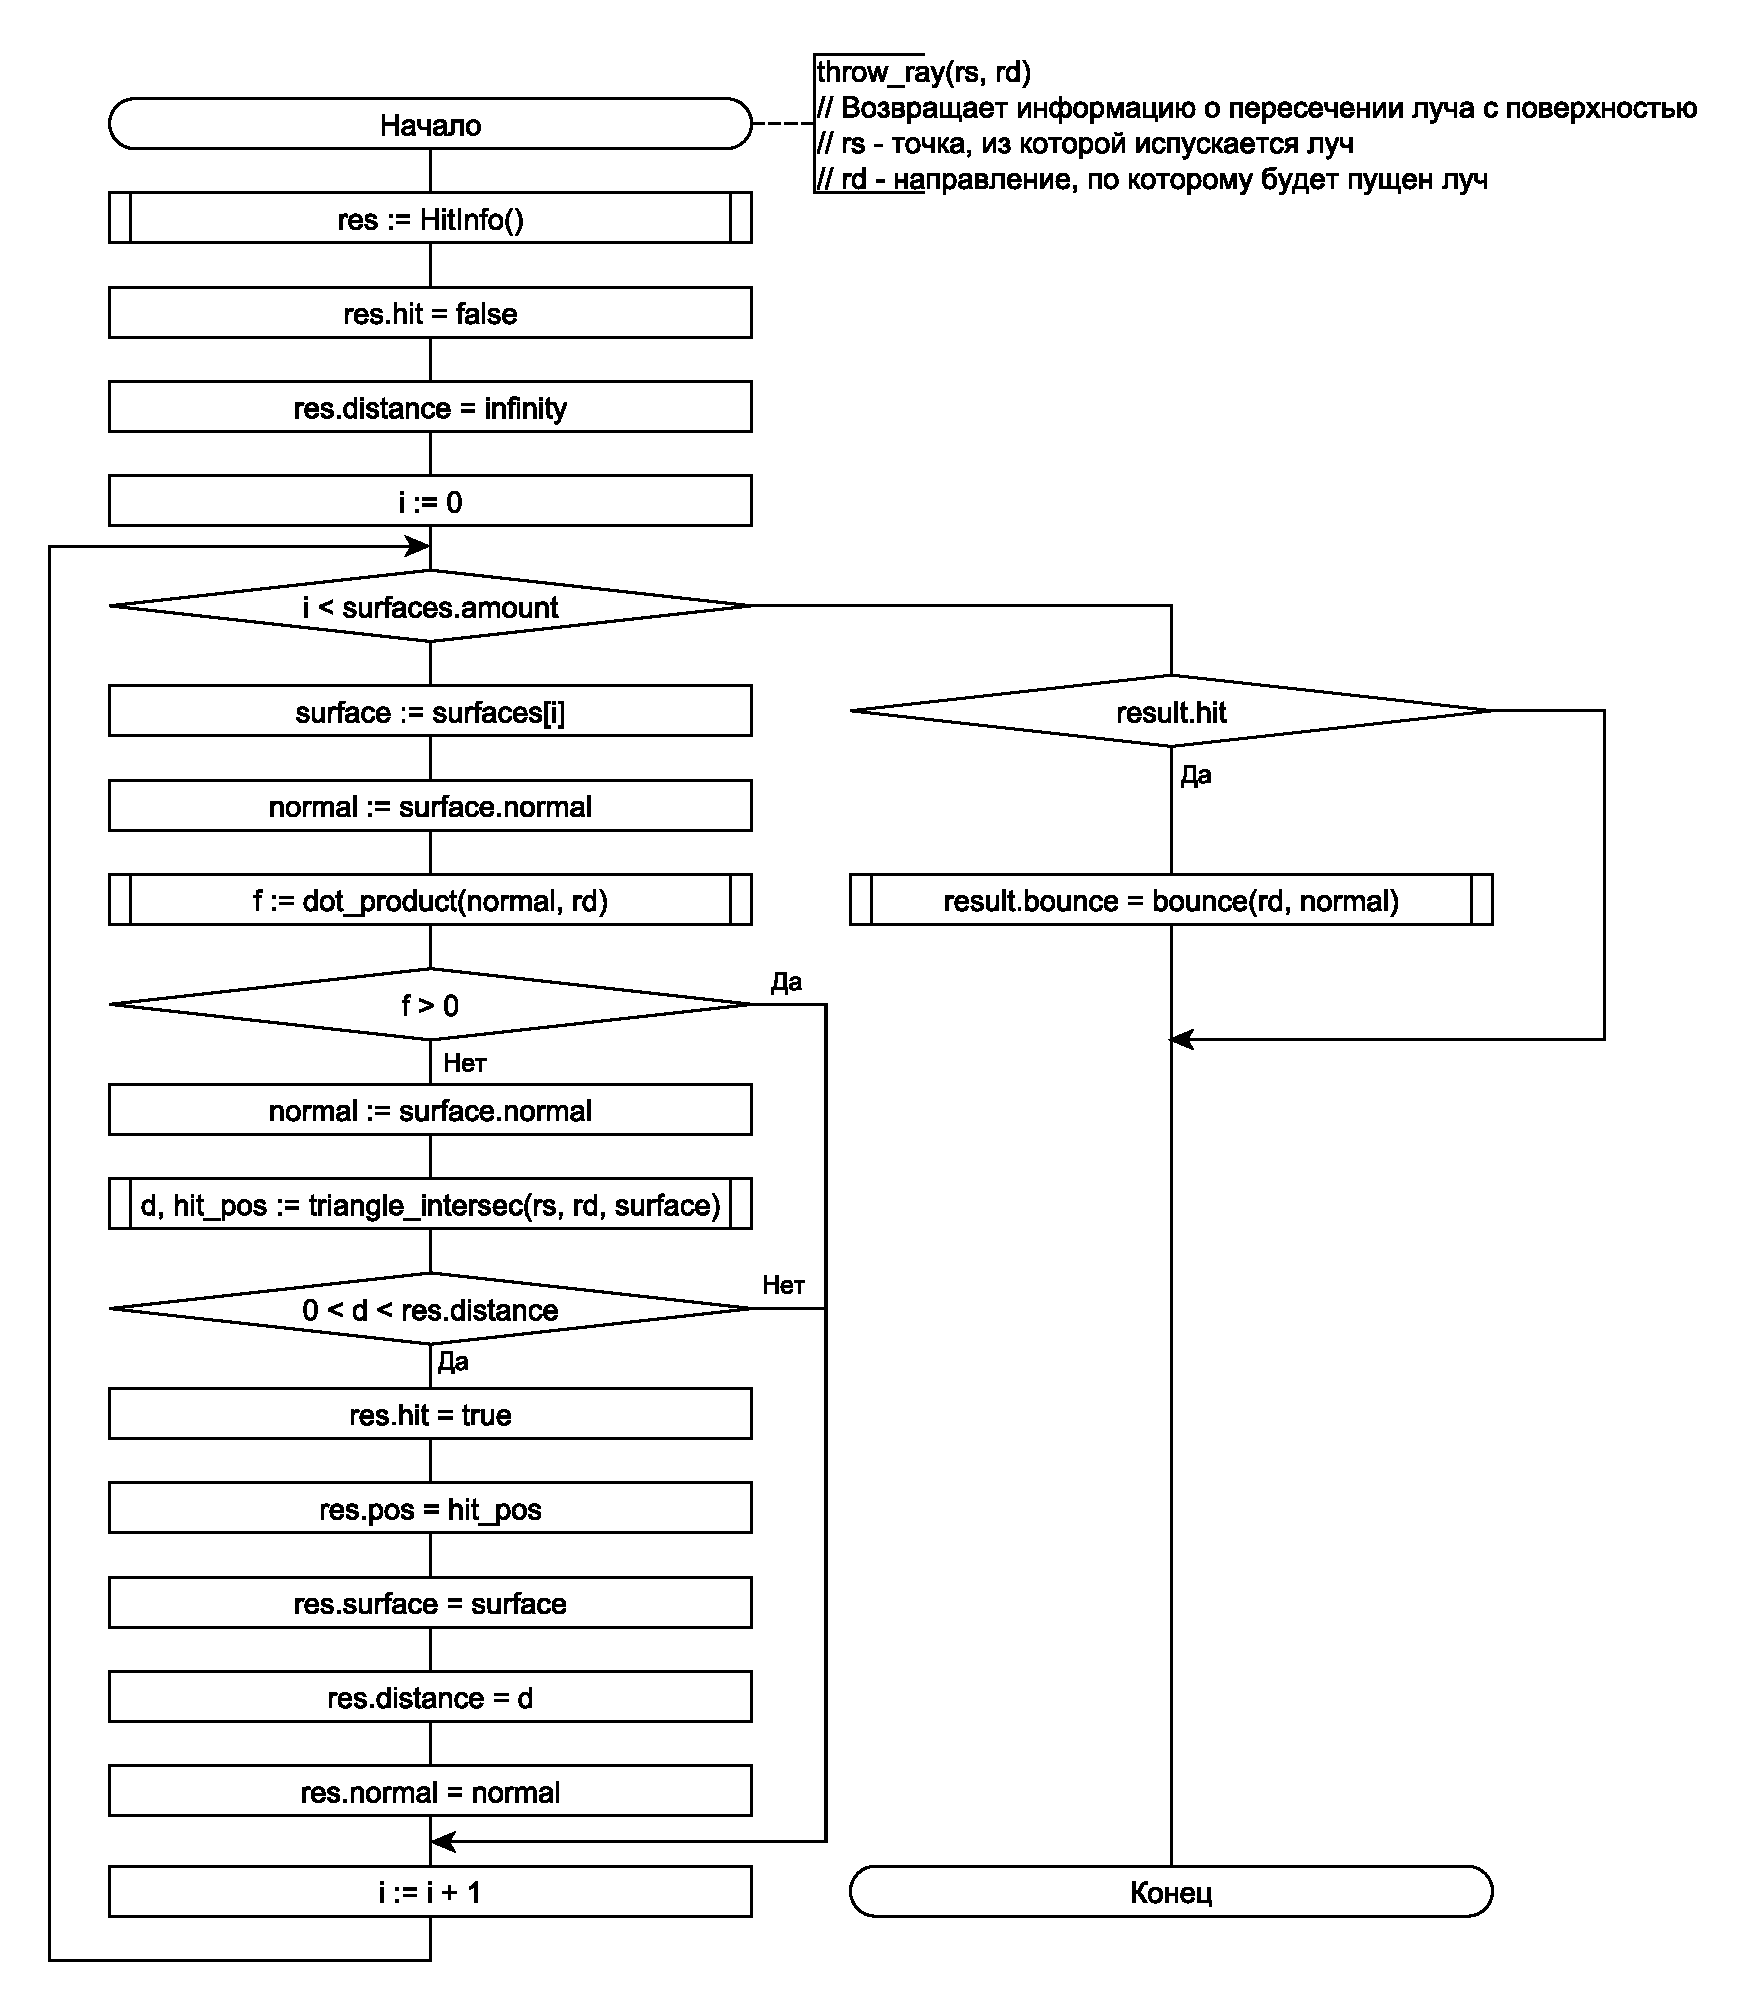
\includegraphics[width=1\linewidth]{throw_ray}}
	\caption{Схема алгоритма бросания луча}
	\label{fig:throw_ray}
\end{figure}

Функция bounce выполняет отражение вектора $\bar V$ относительно нормали $\bar n$ в соответствии с формулой \ref{eq:bounce}

\subsubsection{Алгоритм поиска пересечения луча с треугольником}
В качестве алгоритма поиска пересечения луча с треугольником используется алгоритм Моллера-Трумбора\cite{bib:mollertrumbor}. Схема алгоритма представлена на рис. \ref{fig:triangle_intersec}
\begin{figure}[!ht]
	\center{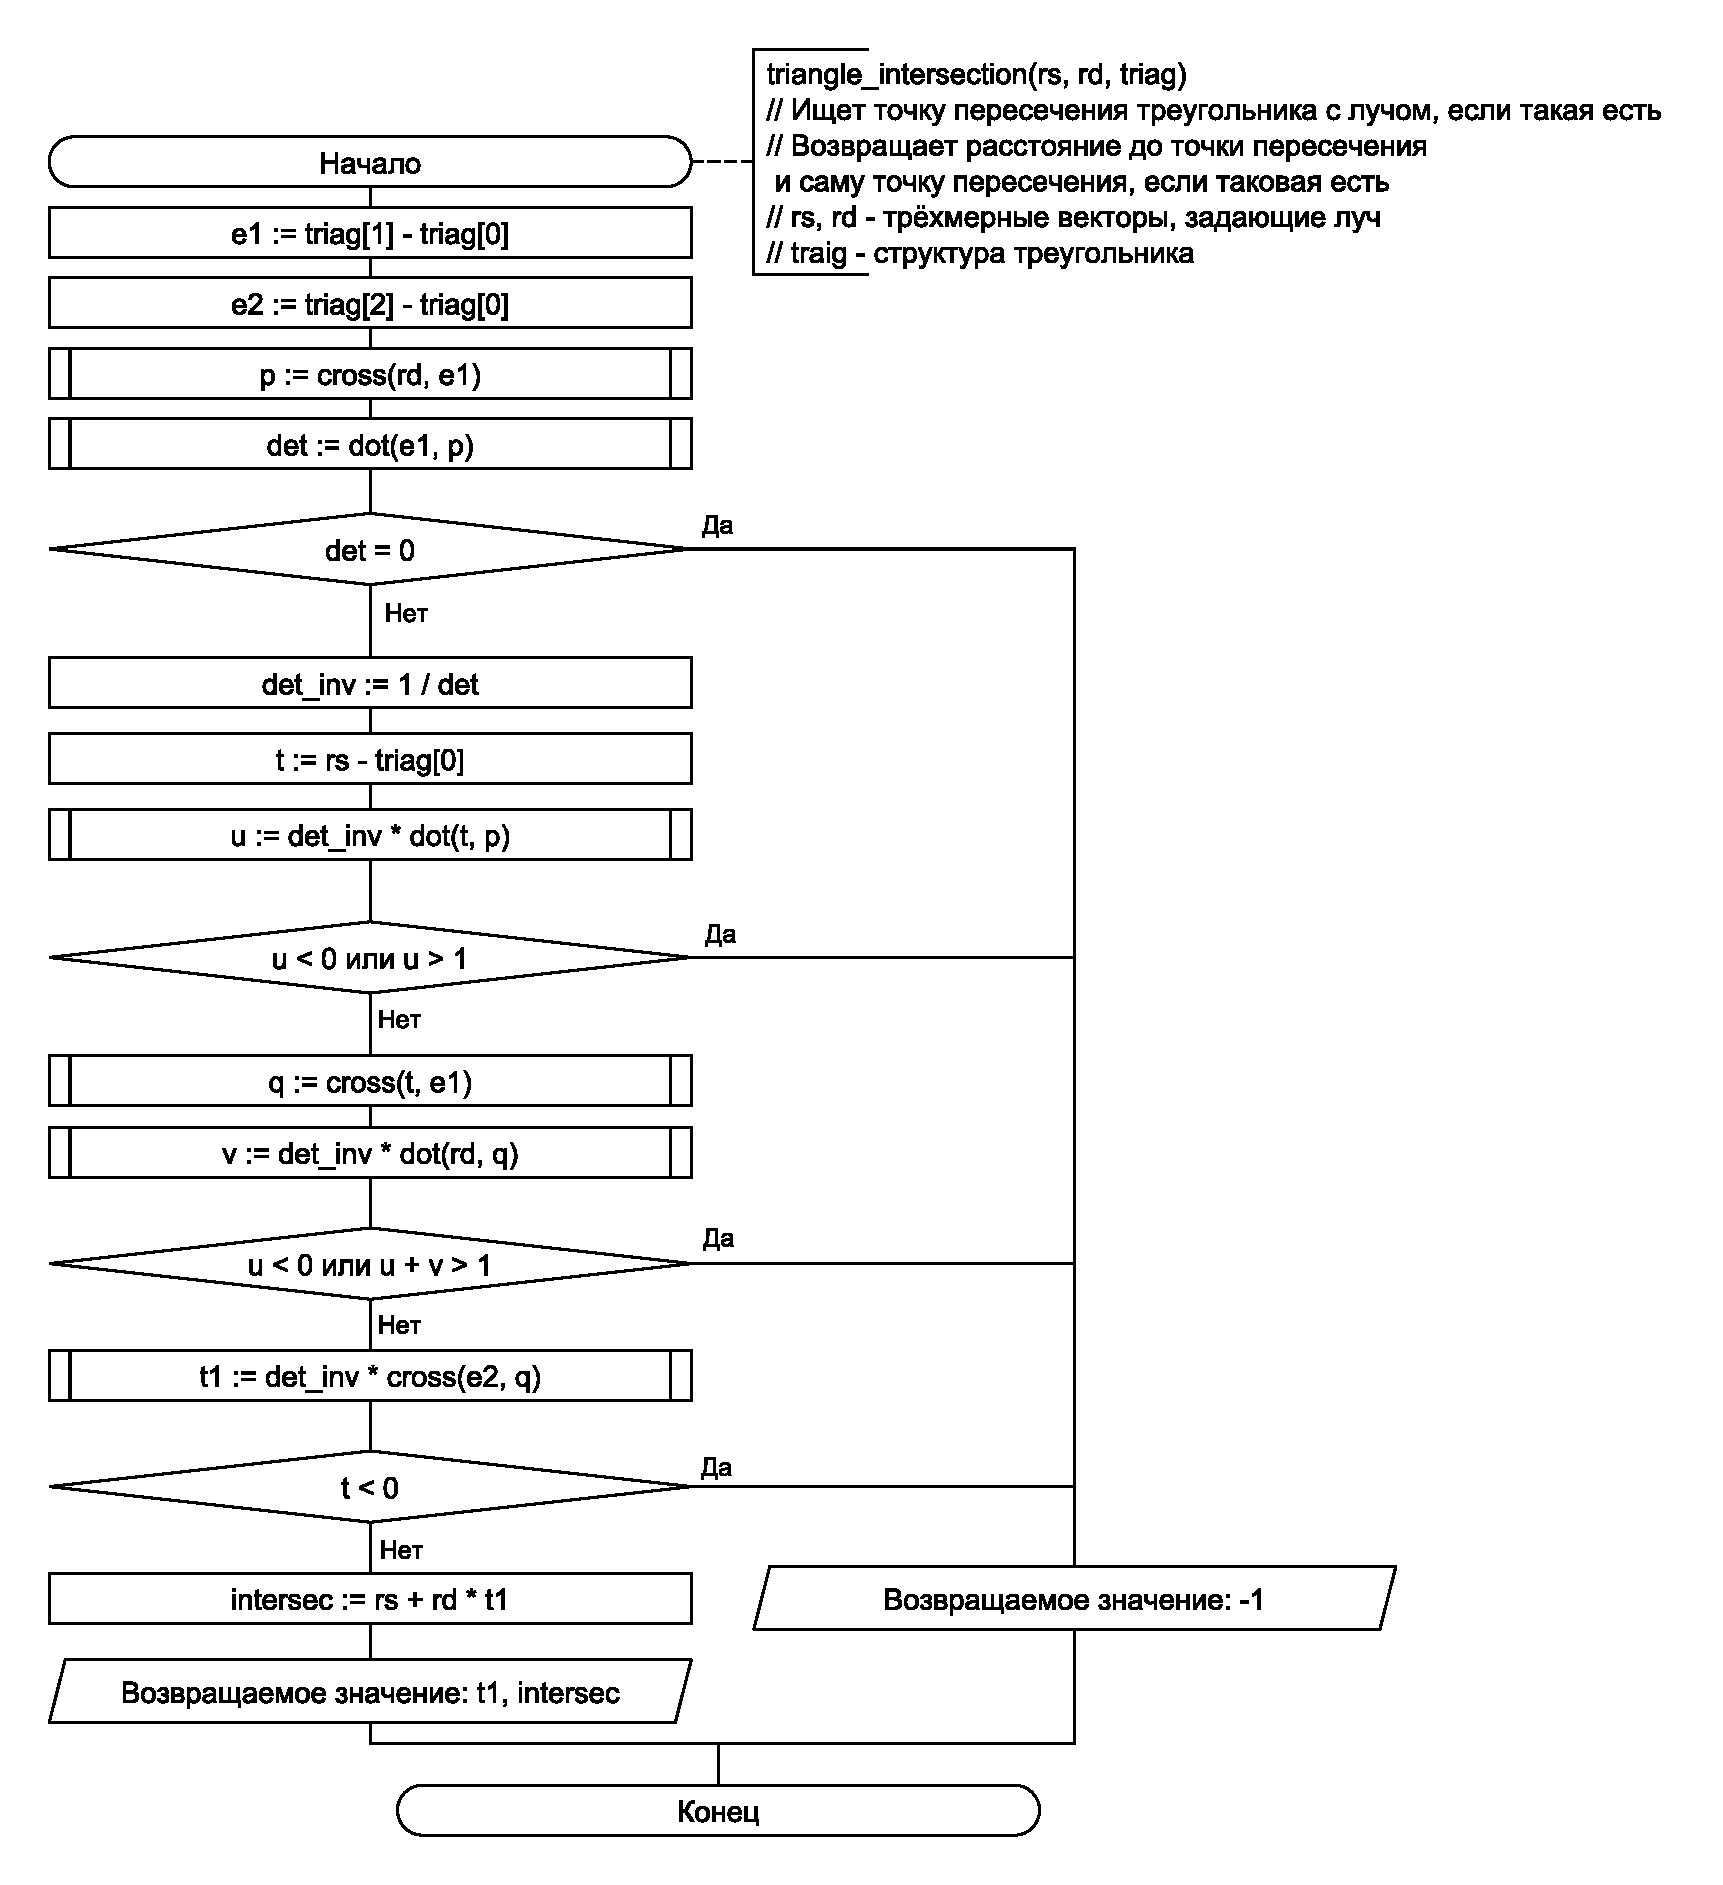
\includegraphics[width=1\linewidth]{triangle_intersec}}
	\caption{Схема алгоритма поиска пересечения луча с треугольником}
	\label{fig:triangle_intersec}
\end{figure}

Функция cross выполняет векторное произведение двух векторов по формуле:
\begin{equation}
	(x_1, y_1, z_1)\times(x_2, y_2, z_2)=(y_1\cdot z_2-z_1\cdot y_2,~z_1\cdot x_2-x_1\cdot z_2,~x_1\cdot y_2-y_1\cdot x_2)
\end{equation}

Функция dot вычисляет скалярное произведение двух векторов по формуле:
\begin{equation}
	(x_1, y_1, z_1)\cdot(x_2, y_2, z_2) = x_1\cdot x_2+y_1\cdot y_2+z_1\cdot z_2
\end{equation}

Идея алгоритма заключается в том, чтобы отыскать точку пересечения луча с треугольником в барицентрических координатах. Вместо того, чтобы искать точку пересечения луча и плоскости, а потом определять лежит ли точка внутри треугольника, получив барицентрические координаты по их значению можно сразу понять, лежит ли точка внутри треугольника или нет

\subsection{Зеркальный кубик Рубика}
Создавать зеркальный кубик Рубика необходимо в соответствии с пропорциями, указанными на рис. \ref{fig:mirrored_cube_proportions}. Схема алгоритма создания параллелограммов представлена на рис \ref{fig:rubicks_create}. Данная схема не иллюстрирует использование пропорций, и отражает лишь порядок в котором должны создаваться параллелограммы.

\subsubsection{Вращение зеркального кубика Рубика}

Вращение грани производится в три этапа (порядок произвольный):
\begin{enumerate}
	\item вращение моделей,
	\item смещение граней в массиве,
	\item смещение углов в массиве.
\end{enumerate}

\begin{figure}[!ht]
	\center{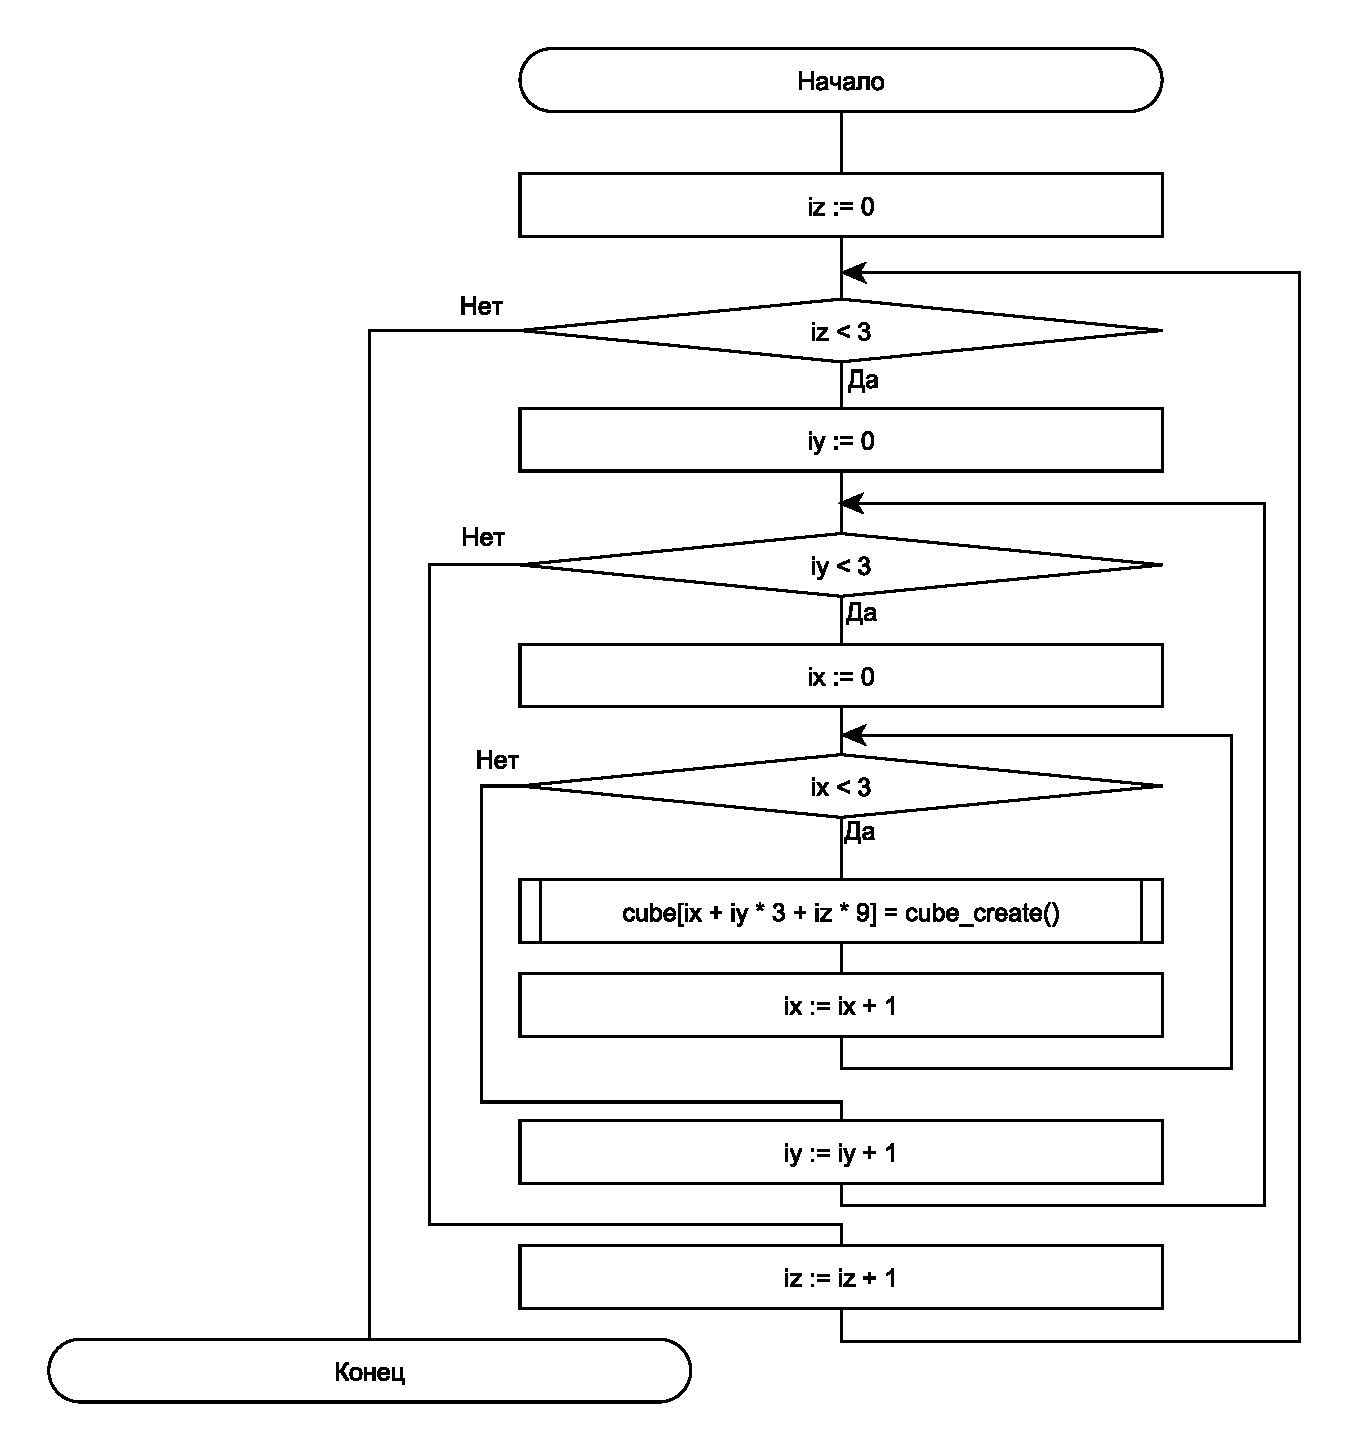
\includegraphics[width=0.78\linewidth]{rubicks_create}}
	\caption{Схема алгоритма создания кубика рубика}
	\label{fig:rubicks_create}
\end{figure}
\begin{table}[!ht]
	\centering
	\caption{грани кубика Рубика и соответствующие им параллелограммы}
	\label{tabular:cube_indexes}
	\begin{tabular}{|c|c|c|}
		\hline
		Сторона & Индексы углов & Индексы граней \\
		\hline
		\hline
		F & 0, 6, 24, 18	& 3, 15, 21, 9		\\ \hline
		B & 8, 2, 20, 26	& 5, 11, 23, 17		\\ \hline
		L & 6, 8, 26, 24	& 7, 17, 25, 15		\\ \hline
		R & 2, 0, 18, 20	& 1, 9, 19, 11		\\ \hline
		U & 18, 24, 26, 20	& 21, 25, 23, 19	\\ \hline
		D & 0, 2, 8, 6		& 1, 5, 7, 3		\\ \hline
	\end{tabular}
\end{table}

Под углами и гранями подразумеваются угловые и граневые параллелограммы кубика Рубика.

Смещение граней и углов в массиве выполняется как циклический сдвиг его элементов с соответствующей четвёркой индексов. В таблице \ref{tabular:cube_indexes} поставлены в соответствие какой циклический сдвиг нужно сделать при повороте соответствующей грани. Если вращение выполняется в противоположную сторону, достаточно развернуть последовательность индексов в другую сторону.

\subsection{Вывод по разделу}
В конструкторском разделе была описана архитектура создаваемой программы;
выделены структуры, используемые в программе;
ключевые алгоритмы, в числе которых отрисовка сцены методом трассировки лучей,
поиск точки пересечения луча и треугольника, вращение кубика Рубика.


\section{Технологический раздел}
В технологическом разделе будет рассмотрен подход к реализации программы, представлен внешний вид интерфейса. Также будут перечислен набор тестовых данных для некоторых функций программы.

\subsection{Выбор используемых технологий}
Далее будут представлены используемые технологии, и обоснован их выбор.

\subsubsection{Выбор ЯП}
Основные два требования, которые предъявляются к языку программирования в рамках поставленной задачи:
\begin{enumerate}
	\item высокая производительность;
	\item поддержка ООП;
	\item наличие средств профилирования;
	\item существование библиотек для замера времени.
\end{enumerate}

Всем перечисленым выше требованиям отвечает язык <<С++>> стандарта 20-го года \cite{bib:cpp_oop}.

\subsubsection{Выбор фреймворка}
Одно из ограничений курсовой работы --- запрет на использование уже существующих решений для отрисовки трёхмерной сцены. Так как алгоритм будет разрабатываться самостоятельно, производительность не является основным критерием для выбора фреймворка. От него требуется возможность отрисовать на экране сетку пикселей. Также фреймворк должен предоставлять средства разработки графического интерфейса.

Всем вышеперечисленым требованиям удовлетворяет пакет программ <<Qt>>, он и будет использоваться для создания интерфейса и отрисовки сетки пикселей на экране \cite{bib:qt_framework}.

\subsubsection{Выбор среды программирования}
Qt creator --- кроссплатформенная среда разработки, разработана специально для работы с фреймворком Qt. Несмотря на это, в качестве среды программирования (далее IDE) был использован Microsoft Visual Studio 2020. Таков выбор объясняется тем, что данная IDE предоставляет \cite{bib:visual_studio}:

\begin{itemize}
	\item систему решений, позволяющих разделять программуна множество связанных между собой проектов
	\item средства профилирования, графически выделяющие строчки кода, занимающие большую долю процессорного времени
	\item средства упрощённой работы с git
\end{itemize}

Таким образом, в качестве IDE используется Microsoft Visual Studio 2020

\subsection{Интерфейс пользователя}
Интерфейс программы представлен на рисунке \ref{fig:interface}.

\begin{figure}[ht]
	\centering
	\includegraphics[width=1\linewidth]{interface}
	\caption{Интерфейс программы}
	\label{fig:interface}
\end{figure}

Справа находится окно просмотра, в котором отображается сцена после отрисовки. Основные элементы управления программой находятся слева.

\subsubsection{Кнопки, флаги, поля}
Кнопки U, L, F, R, D, B выполняют соответствующий поворот зеркального кубика Рубика, по отношению к изначальной позиции камеры. Флаг Пр. Ч. С. переключает кнопки U, L, F, R, D, B на U', L', F', R', D', B', функция которых меняется в соответствии с названием.

Список поворотов --- поле только для чтения, в которое записывается каждый совершённый поворот.

Пикселей на луч --- числовое поле, позволяющее установить габариты квадрата из пикселей, для которого будет пущен луч. Например, при значении 3, на каждый луч будет приходиться $3\times 3$ пикселей.

Автоматическая отрисовка --- флаг, при включении которого любое действие меняющее сцену или область отрисовки будет инициировать автоматическую перерисовку.

Отрисовать --- кнопка, инициирующая рендер сцены.

\subsubsection{Меню}
Меню Куб предоставляет действия:
\begin{enumerate}
	\item Отменить поворот. Переводит куб в состояние, в котором он был до последней операции поворота грани
	\item В исходное состояние. Переводит куб с состояние, в котором он был при запуске программы
\end{enumerate}

Меню Сцена предоставляет действие <<Простая отрисовка>>. Переключает программу между режимами отрисовки сцены с использованием алгоритмов трассировки лучей и проецирования каркасной модели без удаления невидимых граней.

Меню Камера предоставляею опцию <<В исходное состояние>>, которая возвращает камеру на позицию, где она была в момент запуска программы.

Кроме того, в меню камера содержится подменю <<Повернуть...>> в котором перечислены 4 действия, смещающие камеру:
\begin{enumerate}
	\item Влево
	\item Вправо
	\item Вверх
	\item Вниз
\end{enumerate}

\subsection{Тестирование}
Для тестирования методов, работающих с математическими структурами, используется система автоматического тестирования Microsoft Visual Studio CPP Unit Test Framework. На листинге \ref{lst:testcode} представлен пример тестирующего метода.

TEST\_CLASS --- группа тестов, соответствующая классу программы; TEST\_METHOD --- метод, в котором прописаны тесты для соответствующего тестируемого метода класса. Для прогонки тестов используется окно <<Test Explorer>>. Его внешний вид представлен на рис \ref{fig:test_explorer}.

\begin{figure}[ht]
	\centering
	\includegraphics[width=1\linewidth]{img/test_explorer}
	\caption{Окно Test Explorer}
	\label{fig:test_explorer}
\end{figure}
\clearpage

\begin{lstlisting}[caption={Класс, реализующий тестирование методов для работы с трёхмерным вектором},label={lst:testcode},language=c++]
#include "pch.h"
#include "CppUnitTest.h"

using namespace Microsoft::VisualStudio::CppUnitTestFramework;

namespace unittest {	
	TEST_CLASS(TestVector3D) {
		public:
		TEST_METHOD(DotProduct) {
			Assert::AreEqual(Vector3D(4,-6,2)*Vector3D(2,3,3),-4.);
			Assert::AreEqual(Vector3D(2,3,3)*Vector3D(4,-6,2),-4.);
			Assert::AreEqual(
			Vector3D::dot_product(Vector3D(4,-6,2),Vector3D(0,0,0)),0.);
			Assert::AreEqual(
			Vector3D::dot_product(Vector3D(2,3,3),Vector3D(4,-6,2)),0.);
		}
		TEST_METHOD(CrossProduct) {
			auto a = Vector3D(4, -6, 2);
			auto b = Vector3D(2, 3, 3);
			Vector3D cross = Vector3D::cross_product(a, b);
			Assert::AreEqual(Vector3D(-24, -8, 24).to_string(), cross.to_string());
			b = Vector3D(0, 0, 0);
			cross = Vector3D::cross_product(a, b);
			for (int i = 0; i < 3; i++)
			Assert::AreEqual(0., cross[i]);
		}
	};
}
\end{lstlisting}

\subsubsection{Тестовые данные}
Далее будут приведены данные, использованные для тестирования функций, работающих с основными структурами.

Структура угла (Angle):
\begin{enumerate}
	\item real Angle::to\_radians(real) --- функция, принимающая на вход значение угла в градусах, возвращающая значение угла в радианах. Тестовые данные приведены в таблице \ref{tbl:to_radians}.
	\item real Angle::to\_degrees(real) --- функция, принимающая на вход значение угла в радианах, возвращающая значение угла в градусах. Тестовые данные приведены в таблице \ref{tbl:to_radians}.
	\begin{table}[!ht]
		\centering
		\caption{Тестовые данные для функций real Angle::to\_radians(real) и real Angle::to\_degrees(real)}
		\label{tbl:to_radians}
		\begin{tabular}{|c|c|l|}
			\hline
			Угол в градусах & Угол в радианах & Класс эквивалентности \\
			\hline
			180	& $\pi$	& Половина окружности \\
			90	& $\frac{\pi}{2}$ & Произвольный случай \\
			45	& $\frac{\pi}{4}$ & Произвольный случай \\
			-90 & $-\frac{\pi}{2}$ & Отрицательный угол \\
			0	& 0 & Нулевой угол \\
			\hline
		\end{tabular}
	\end{table}
	
	\item real Angle::optimize\_degrees(real) --- функция, приводящий произвольный угол $\alpha\in\mathbb{R}$, заданный в градусах к углу $\beta\in\left[0; 360\right)$, заданному в градусах. Тестовые данные для этой функции приведены в таблице \ref{tbl:optimize_radians}
	\begin{table}[!ht]
		\centering
		\caption{Тестовые данные для функции Angle::optimize\_degrees(real)}
		\label{tbl:optimize_radians}
		\begin{tabular}{|c|c|l|}
			\hline
			Вход & Выход & Класс эквивалентности \\
			\hline
			$\frac{5\pi}{2}$ & $\frac{\pi}{2}$ & Больше окружности \\
			$-\frac{\pi}{2}$ & $\frac{3\pi}{2}$	& Отрицательный угол \\
			$\frac{\pi}{2}$ & $\frac{\pi}{2}$ & Уже нормализованный угол \\
			$0$ & $0$ & Нулевой угол\\
			$2\pi$ & $0$ & Ровно окружность\\
			\hline
		\end{tabular}
	\end{table}
	
	\item real Angle::optimize\_degrees(real) --- функция, приводящий произвольный угол $\alpha\in\mathbb{R}$, заданный в радианах к углу $\beta\in\left[0; 2\pi\right)$, заданному в радианах. Тестовые данные для этой функции приведены в таблице \ref{tbl:optimize_degrees}
	\begin{table}[!ht]
		\centering
		\caption{Тестовые данные для функции Angle::optimize\_degrees(real)}
		\label{tbl:optimize_degrees}
		\begin{tabular}{|c|c|l|}
			\hline
			Вход & Выход & Класс эквивалентности \\
			\hline
			540 & 180 & Больше окружности\\
			-90 & 270 & Отрицательный угол\\
			90 & 90 & Уже нормализованный угол\\
			0 & 0 & Нулевой угол\\
			360 & 0 & Ровно окружность\\
			\hline
		\end{tabular}
	\end{table}
\end{enumerate}

\subsubsection{Окно просмотра}
Оценка правильности полученного изображения была проведена с помощью визуального анализа. В качестве вспомогательного инструмента, была реализована функция отображения сцены в каркасном виде без удаления граней. Внешний вид окна просмотра при работе этой функции представлен на рис. \ref{fig:scenecarcass}

\begin{figure}[ht]
	\centering
	\includegraphics[width=0.7\linewidth]{img/scene_carcass}
	\caption{Окно просмотра в режиме простой отрисовки}
	\label{fig:scenecarcass}
\end{figure}

\subsection{Вывод по разделу}
В технологическом разделе представлены все использованные программные средства с обоснованием их выбора, а именно:
\begin{itemize}
	\item C++ стандарта 20-го года;
	\item Qt фреймворк;
	\item Microsoft Visual Studio 2020;
\end{itemize}

Представлены методы тестирования программы, тестовые данные и описан интерфейс пользователя.


\section{Исследовательский раздел}
В исследовательском разделе будут проведены замеры времени для разных конфигураций камеры и зеркального кубика рубика. В дальнейшем, такая конфигурация будет называться кадром.

\subsection{Характеристики ПК}
Все дальнейшие замеры времени будут проведены на настольном персональном компьютере, имеющем характеристики:
\begin{itemize}
	\item процессор --- AMD Ryzen 7 1700X, 3.4 ГГц \cite{bib:processor};
	\item ОЗУ --- 16ГБ DDR4-2133, 1066 МГц;
	\item видеокарта --- AMD Radeon RX 570, 8 Гб GDDR5, ядро 1250 МГц, память 1750 МГц \cite{bib:graphics-card}.
\end{itemize}

\subsection{Результаты измерения времени}
В таблице \ref{tbl:time_measures} представлены результаты замеров времени, проведённых для кадров, представленных на рисунках \ref{fig:test1}, \ref{fig:test2}, \ref{fig:test3}, \ref{fig:test4}, \ref{fig:test5} и \ref{fig:test6} соответственно.

\begin{table}[!ht]
 	\centering
 	\caption{Результаты замеров времени}
 	\label{tbl:time_measures}
 	\begin{tabular}{|c|c|c|}
 		\hline
 		№ кадра & Число пикселей & Время в миллисекундах \\
 		\hline
 		1 & 1578260 & 52718.7 \\
 		2 & 1578260 & 42159.7 \\
 		3 & 1578260 & 36643.9 \\
 		4 & 1578260 & 56138.4 \\
 		5 & 1578260 & 48544.3 \\
 		6 & 1578260 & 48345.9 \\
 		\hline
 	\end{tabular}
 \end{table}

\begin{figure}
	\centering
	\includegraphics[width=1\linewidth]{test1}
	\caption{Кадр для теста №1}
	\label{fig:test1}
\end{figure}

\begin{figure}
	\centering
	\includegraphics[width=1\linewidth]{test2}
	\caption{Кадр для теста №2}
	\label{fig:test2}
\end{figure}

\begin{figure}
	\centering
	\includegraphics[width=1\linewidth]{test3}
	\caption{Кадр для теста №3}
	\label{fig:test3}
\end{figure}

\begin{figure}
	\centering
	\includegraphics[width=1\linewidth]{test4}
	\caption{Кадр для теста №4}
	\label{fig:test4}
\end{figure}

\begin{figure}
	\centering
	\includegraphics[width=1\linewidth]{test5}
	\caption{Кадр для теста №5}
	\label{fig:test5}
\end{figure}

\begin{figure}
	\centering
	\includegraphics[width=1\linewidth]{test6}
	\caption{Кадр для теста №6}
	\label{fig:test6}
\end{figure}

\subsection{Вывод по разделу}
В исследовательском разделе были проведены замеры времени для шести различных кадров. Из полученных результатов можно сделать вывод о том, что наиболее трудоёмким процессом является рассчёт интенсивности света в точке.


\section*{Заключение}
\addcontentsline{toc}{section}{Заключение}
Цель достигнута. В рамках данной курсовой работы были проанализированы существующие алгоритмы отрисовки сцены, среди которых был выбран алгоритм обратной трассировки лучей, из-за возможности отрисовки зеркальных поверхностей.

Была составлена архитектура программы:
\begin{itemize}
	\item представлена сокращённая UML-диаграмма классов сцены (рисунок \ref{fig:uml_scene});
	\item выделены основные используемые программой структуры данных;
	\item формализованы алгоритмы, необходимые для отрисовки сцены.
\end{itemize}

Была реализована программа:
\begin{itemize}
	\item был определён набор инструментов для её реализации;
	\item представлен внешний вид интерфейса (рисунок \ref{fig:interface});
	\item составлены тесты для функций, использующих математические структуры данных.
\end{itemize}

\bibliographystyle{utf8gost705u}
\bibliography{sources}

\addcontentsline{toc}{section}{Приложение А}
\section*{Приложение А}

\end{document}